\chapter{ownCloud}
%---------------------------------------------------------------------------------------------------------------------------------
\section{Introduction}

\noindent Un serveur ownCloud peut être installé de différentes façons \footnote{\url{https://owncloud.org/install/\#instructions-server}} :

\begin{enumerate}
 \item Par le gestionnaire de package de votre système (ex : apt-get)
 \item En lançant une image cloud déjà configurée (disponible sur Azure, Google Cloud, Amazon AWS, Juju)
 \item Avec un web installer (fichier PHP à télécharger)
 \item Avec l'archive d'ownCloud
\end{enumerate}


Nous allons utiliser ici la quatrième façon, c'est-à-dire une installation depuis l'archive officielle d'ownCloud. Cette technique nous permet d'être plus libre, de pouvoir gérer soit-même les mises à jour et de modifier le code source si nécessaire. Par contre il y a des inconvénients. Nous avons l'obligation de tout installer depuis zéro (services, base de données, serveur, réseau, autorisations, etc.).

Nous allons à présent pouvoir installer ownCloud serveur sur notre instance. La procédure expliquée ci-bas est tirée de la page suivante : 
\url{https://doc.owncloud.org/server/8.0/admin_manual/installation/source_installation.html}. Il s'agit du manuel d'installation d'ownCloud Sever 8.

%---------------------------------------------------------------------------------------------------------------------------------
\section{Installation}

\subsection{Mise à jour des packages de la distribution}

Avant de commencer, il est préférable de mettre à jour la liste des packages disponibles sur votre instance Ubuntu et de mettre à jour les logiciels. Voici les deux commandes à exécuter : \\

\begin{lstlisting}[language=bash]
  sudo apt-get update
  sudo apt-get upgrade
\end{lstlisting}

\subsection{Installation de PHP et MariaDB}

Il faut installer PHP ainsi que la base de données MariaDB : \\

\begin{lstlisting}[language=bash]
  sudo apt-get install apache2 mariadb-server libapache2-mod-php5
  sudo apt-get install php5-gd php5-json php5-mysql php5-curl
  sudo apt-get install php5-intl php5-mcrypt php5-imagick
\end{lstlisting}

Lors de l'installation, l'assistant vous demande si vous voulez vraiment installer les packages, tapez simplement ``Y'' (pour Yes). Ensuite MariaDB demande un mot de passe pour l'utilisateur root. Choisissez-en un et mémorisez-le.


\subsection{Téléchargement de l'archive ownCloud}

Il faut à présent télécharger l'archive ownCloud. Pour cela il y a différentes façon. La première est de suivre de lien \url{https://owncloud.org/install/}, de cliquer sur \texttt{Download} et de télécharger l'archive \texttt{.tar.bz2} ou \texttt{.zip}. Il faudra ensuite envoyer cette archive sur votre instance pour l'utiliser. Dans ce cas, vous accéderez à la dernière version stable d'ownCloud server. La seconde façon est de télécharger l'archive directement depuis votre instance. Il faudra savoir le numéro de version voulue et la remplacer dans le lien ci-dessous. Voici comment le faire : \\

\begin{lstlisting}[language=bash]
  wget https://download.owncloud.org/community/owncloud-8.0.3.tar.bz2
\end{lstlisting}

A partir de là, la stratégie est la même dans les deux cas : il faut désarchiver (dézipper) le fichier : \\

\begin{lstlisting}[language=bash]
  sudo tar -xjvf owncloud-8.0.3.tar.bz2 
\end{lstlisting}

Il faut ensuite copier le dossier \texttt{owncloud} à la racine du serveur Apache : \\

\begin{lstlisting}[language=bash]
  sudo cp -r owncloud /var/www/
\end{lstlisting}

\subsection{Configuration du serveur Apache}

Nous voulons créer un fichier de configuration Apache pour ownCloud, voici la recette : \\

\begin{lstlisting}[language=bash]
  cd /etc/apache2/conf-available/
  sudo touch owncloud.conf
  sudo vim owncloud.conf
\end{lstlisting}

Nous nous trouvons alors dans VIM, il faut écrire les lignes suivantes dans le fichier \texttt{owncloud.conf} : \\

\begin{lstlisting}[language=bash]
  Alias /owncloud /var/www/owncloud
  <Directory /var/www/owncloud/>
     AllowOverride All
     Satisfy Any
  </Directory>
\end{lstlisting}

% s'il y a un WebDAV sur le serveur, il faut le désactiver en ajoutant ``Dav Off'' dans ``<Directory''

Et pour que le fichier soit pris en compte, on ajoute un lien symbolique dans le bon dossier : \\

\begin{lstlisting}[language=bash]
  sudo ln -s /etc/apache2/conf-available/owncloud.conf /etc/apache2/conf-enabled/owncloud.conf
\end{lstlisting}

Il faut également activer le mode \texttt{rewrite} sur Apache (et redémarrer Apache pour que le changement soit pris en compte) : \\

\begin{lstlisting}[language=bash]
  sudo a2enmod rewrite
  service apache2 restart
\end{lstlisting}

% ATTENTION A CA :
  % When using SSL, take special note on the ServerName. 
  % You should specify one in the server configuration, 
  % as well as in the CommonName field of the certificate. 
  % If you want your ownCloud to be reachable via the internet, 
  % then set both of these to the domain you want to reach your ownCloud server.
  
  
Notre serveur Apache est correctement installé. Pour en être sûr, accédez à votre instance par HTTP en insérant l'IP de l'instance dans un navigateur. Attention, pour que ça fonctionne il faut avoir ajouté une règle pour le HTTP dans le \texttt{Security Group} lié à votre instance. Si tout fonctionne, vous verrez la page de la figure \ref{apacheisworking} s'afficher.


\begin{figure}[h]
  \centering
    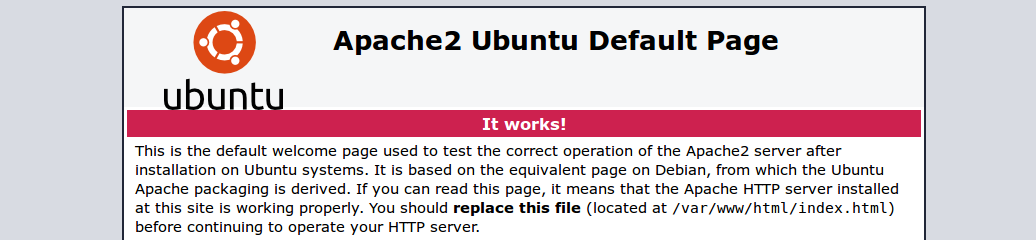
\includegraphics[width=\linewidth]{img/apacheIsWorking.png}
  \caption{Page d'accueil du serveur Apache}
  \label{apacheisworking}
\end{figure}

\section{Gestion des droits}

Pour accéder à l'interface web d'ownCloud server, il suffit d'ajoute ``\texttt{/owncloud}`` à la fin de l'IP de l'instance dans le navigateur. A l'état actuel, ownCloud n'a pas les droits corrects pour pouvoir écrire sur le disque comme on peut le voir sur la figure \ref{nowriteaccess}.

\begin{figure}[h]
  \centering
    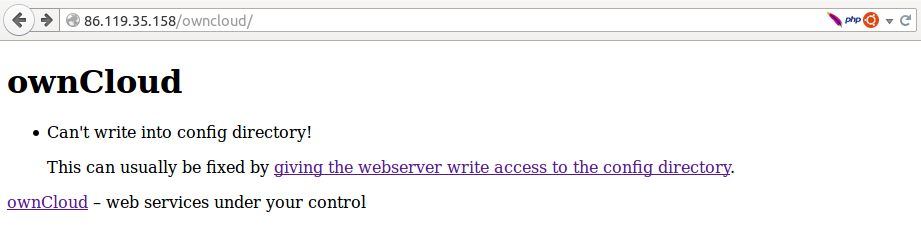
\includegraphics[width=\linewidth]{img/OCWriteAccess.png}
  \caption{OwnCloud n'a pas les droits d'écriture dans le dossier de configuration}
  \label{nowriteaccess}
\end{figure}

Il faut donc que vous lanciez le scipt ci-dessous en mode root après l'avoir déplacé sur l'instance : \texttt{sudo ./changeWriteAccessOC.sh}

\lstinputlisting[language=Python]{code/changeWriteAccessOC.sh}

Rafraîchissez la page web pour voir le résultat (figure \ref{ocwelcomepage}).
% http://86.119.35.158/owncloud/

\begin{figure}[h]
  \centering
    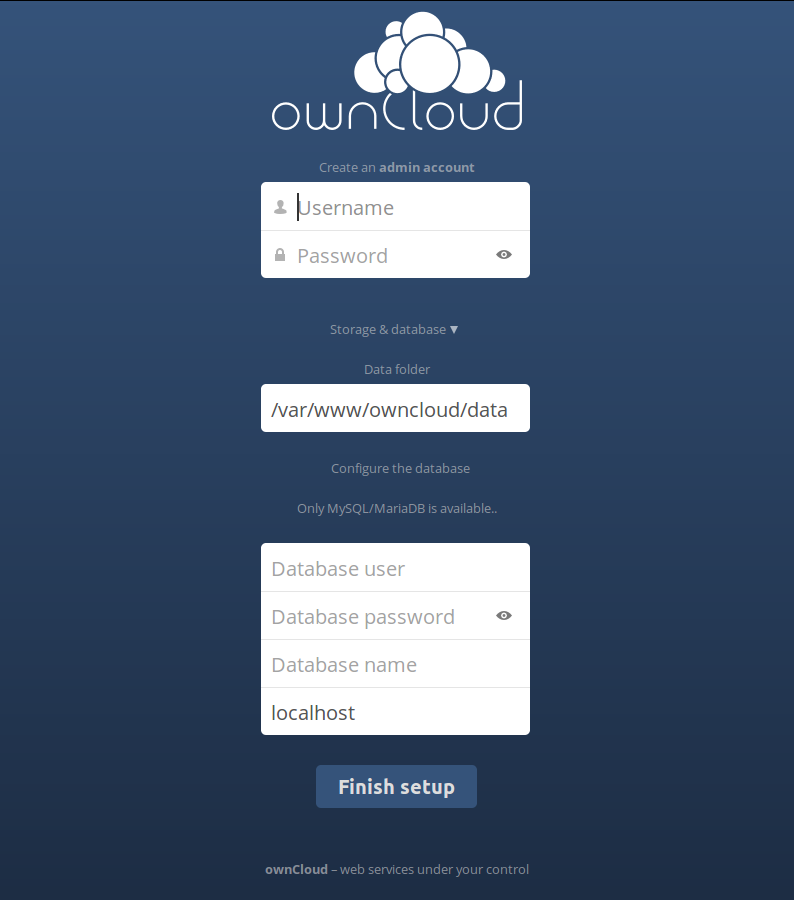
\includegraphics[width=0.8\linewidth]{img/OCWelcomePage.png}
  \caption{ownCloud - Page d'accueil}
  \label{ocwelcomepage}
\end{figure}

\clearpage
\section{Création du compte administrateur}

Sur cette page web, qui est l'administration du serveur ownCloud, il faut à présent créer un compte administrateur et configurer la base de données en entrant des identifiants que vous avez créé précédemment.

\vspace{0.4cm}

\noindent NB : Si un message d'erreur indique que vous ne pouvez pas écrire dans le dossier, il faut créer le dossier puis changer les droits d'écriture de ce celui-ci ainsi que l'attribuer à l'utilisateur 'www-data' pour que l'administration puisse y accéder : \\

\begin{lstlisting}[language=bash]
  cd /var/www
  sudo chmod 755 owncloud
  
  cd /var/www/owncloud
  sudo mkdir data
  sudo chmod 766 data

  sudo chown www-data:www-data -R /var/www/owncloud/data
\end{lstlisting}

Si tout fonctionne correctement, vous serez dirigé vers le dashboard de votre compte ownCloud fraîchement créé (figure \ref{ocdashboard}). On peut voir que deux dossiers et un fichier ont déjà été créés.

\begin{figure}[h]
  \centering
    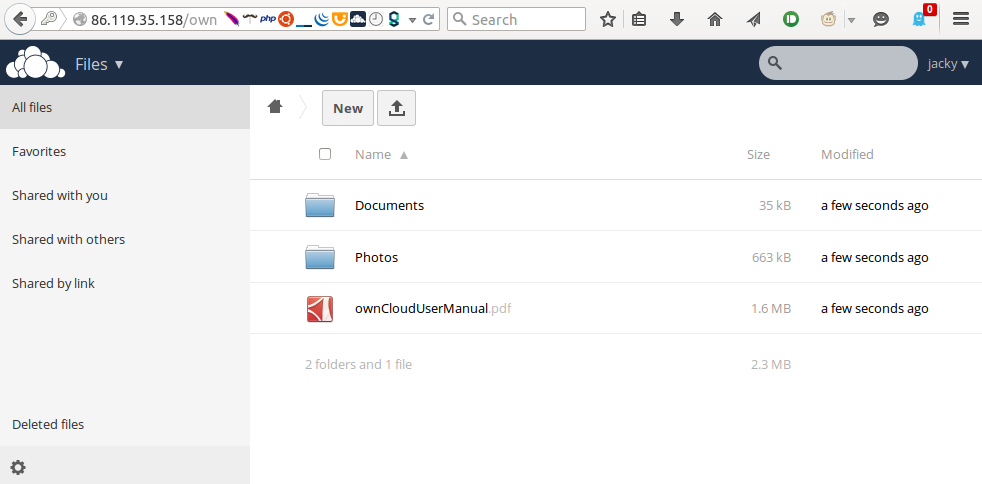
\includegraphics[width=\linewidth]{img/OCDashboard.png}
  \caption{ownCloud - Dashboard}
  \label{ocdashboard}
\end{figure}

\newpage

Vous êtes alors l'administrateur de ce serveur ownCloud. Vous pouvez gérer beaucoup de choses depuis l'interface de l'administration. Cette interface vous permet de gérer vos propres documents mais également de créer d'autres utilisateurs. Vous pouvez créer des groupes avec des droits spécifiques et mettre des utilisateurs dans ces groupes. Vous pouvez paramétrer des crons, paramétrer l'envoi d'emails, etc. 

Vos utilisateurs, ainsi que vous, pouvez installer un client ownCloud\footnote{Client desktop : \url{https://owncloud.com/products/desktop-clients/}} sur votre ordinateur (MacOX, Windows, Linux) pour synchroniser vos fichiers sur le serveur. Il existe également des application smartphone pour Android\footnote{Client Android : \url{https://play.google.com/store/apps/details?id=com.owncloud.android&hl=fr}} et iOS\footnote{Client iOS : \url{https://itunes.apple.com/fr/app/owncloud/id543672169?mt=8}}. Après l'installation, il suffit d'indiquer l'adresse du serveur, le nom d'utilisateur ainsi que le mot de passe et le tour est joué.\\

Ce guide d'installation d'un serveur ownCloud sur une instance SWITCHengines est terminé.
